\documentclass[11pt]{article}
\usepackage[margin=1in]{geometry}
\usepackage{amsmath,amssymb,graphicx,booktabs,listings,xcolor,hyperref,enumitem}
\usepackage{tcolorbox}
\hypersetup{colorlinks=true,linkcolor=blue!60!black,urlcolor=blue!60!black}
\definecolor{codebg}{RGB}{247,247,245}
\lstset{language=Python,basicstyle=\ttfamily\small,backgroundcolor=\color{codebg},frame=single,framerule=0pt,
  keywordstyle=\color{blue!60!black},commentstyle=\color{gray},stringstyle=\color{green!40!black},
  showstringspaces=false,breaklines=true,columns=fullflexible,xleftmargin=4pt,xrightmargin=4pt}
\newtcolorbox{exercise}[1]{colback=blue!3,colframe=blue!50!black,title={Exercise #1},fonttitle=\bfseries,left=4pt,right=4pt}
\newtcolorbox{checkbox}{colback=green!4,colframe=green!40!black,title={What to compare against},fonttitle=\bfseries,left=4pt,right=4pt}
\newtcolorbox{vocab}{colback=orange!4,colframe=orange!60!black,title={Vocabulary},fonttitle=\bfseries,left=4pt,right=4pt}
\newcommand{\eps}{\varepsilon}
\newcommand{\code}[1]{\texttt{#1}}
\newcommand{\F}{\mathbb{F}}
\title{Validating distillation performance by Monte Carlo:\\ a guide to \code{qmsd.mc\_distill} and the next steps}
\author{prime\_msd project notes for Aanha}
\date{28 October 2026}

\begin{document}
\maketitle
\tableofcontents

\section{Where this fits}

\subsection{The paper}

The paper we are assembling has three parts.

\begin{enumerate}[nosep]
\item \textbf{New codes.} Magic-state distillation codes with overhead exponent
  $\gamma<1$ at $p=7$ (the first ever at that dimension), at $p=17$ and $19$, and the
  Reed--Solomon ladder from $p=23$ to $97$; plus your catalog entries at $p=3,5,7$ and
  the first cataloged codes at $p=11,13$.
\item \textbf{A structural result.} No small $\gamma<1$ code exists for $p\le 13$ in
  the Reed--Muller framework; the weighted-support construction that succeeds at $p=7$
  is the one way around it, and it does not help at $3, 11, 13$.
\item \textbf{An exact performance engine.} Every code in the catalog gets its
  output-error curve, threshold and distillation cost computed exactly rather than
  by the leading-order estimate that papers usually quote.
\end{enumerate}

Every cost and threshold number in part~3 rests on one piece of code,
\code{qmsd/performance.py}. It reproduces a published table to every printed digit,
which is reassuring, but nobody has checked it against an \emph{independent} method,
and nobody anywhere has published a noisy-circuit simulation of any qudit
triorthogonal code. Those two checks are your part of the paper.

\subsection{Your two steps}

\begin{enumerate}[nosep]
\item \textbf{Channel-level Monte Carlo} (this document). Sample the noise model the
  engine assumes, apply the acceptance rule exactly as the engine defines it, and show
  that the sampled output error and acceptance probability land on the engine's
  exact curves. Deliverable: Figure~\ref{fig:curves} with your own points on it, for
  at least four codes, and a short table.
\item \textbf{Circuit-level simulation in \code{sdim}.} Replace the idealised
  channel by a noisy encoding-and-measurement circuit for one or two small codes and
  measure how far the real output error departs from the channel-level curve.
  Deliverable: a notebook and a plot of simulated against predicted performance.
\end{enumerate}

Step~1 is deliberately easy: the sampler is 44 lines, the exact curves are already
computed, and the codes have at most 44 qudits. Its value is that it validates
everything downstream, and that every piece of it (the noise model, the acceptance
test, the two error notions, the statistics) reappears unchanged in step~2. If you
do step~1 carefully, step~2 is mostly circuit construction.

\subsection{Reading this document}

Section~\ref{sec:background} is background you may already know; skim it and come
back for the vocabulary boxes. Section~\ref{sec:model} defines exactly what is being
computed. Section~\ref{sec:codes} gives the three codes and the numbers you must
reproduce. Section~\ref{sec:code} walks through the sampler. Section~\ref{sec:ex}
has ten exercises in order of difficulty; each is preceded by a paragraph saying
what it teaches and followed by a box with the expected answer. Section~\ref{sec:sdim}
is the bridge to the circuit simulation. The appendices are copy-paste snippets.

\section{Background in one page}
\label{sec:background}

\paragraph{Qudits and the field $\F_p$.} A qudit of dimension $p$ (a prime) has
basis states $|0\rangle,\dots,|p-1\rangle$. Its Pauli operators are $X|a\rangle =
|a+1\rangle$ and $Z|a\rangle = \omega^{a}|a\rangle$ with $\omega = e^{2\pi i/p}$,
arithmetic mod $p$. A $Z$-type error on $n$ qudits is $Z^{j_1}\otimes\cdots\otimes
Z^{j_n}$ and is described by the vector $j=(j_1,\dots,j_n)\in\F_p^{n}$. Everything in
this document is linear algebra over $\F_p$, the integers mod $p$.

\paragraph{Magic states and distillation.} Clifford gates (the ones a stabiliser
code can do transversally) are not universal. The missing ingredient is supplied by
\emph{magic states}, specific single-qudit states that, consumed by a Clifford
circuit, implement a non-Clifford gate. Preparing them directly gives a noisy
version. \emph{Distillation} takes $n$ noisy copies, runs a Clifford circuit plus
measurements, and outputs $k$ copies with a much lower error, at the cost of
sometimes rejecting the whole batch. The relevant code family is
\emph{triorthogonal}: a condition on the generator matrix that guarantees the
transversal non-Clifford gate acts as a logical non-Clifford gate, so that the
encoded magic states come out clean.

\paragraph{Codes, stabilisers, syndromes.} A CSS code is given by two matrices over
$\F_p$: one whose rows are $X$-type stabilisers and one whose rows are $Z$-type
stabilisers. For distillation only the $Z$ errors matter (the magic state's noise,
after \emph{twirling}, is pure $Z$ noise), and the stabilisers that detect them are the
rows of $G_0$. Measuring a stabiliser row $g$ on an error $j$ returns the
\emph{syndrome} $g\cdot j \bmod p$. All syndromes zero means ``looks clean''. The
\emph{logical operators} are rows $h_i$ that commute with the stabilisers; $h_i\cdot
j\neq 0$ means output $i$ is corrupted.

\paragraph{Distance and overhead.} The \emph{distance} $d$ is the smallest number of
qudits an undetected error can occupy. An error of \emph{weight} $w$ (number of
nonzero entries of $j$) with $w<d$ either triggers a syndrome or is harmless; so
the output error scales as $\eps^{d}$. Using a code recursively, the number of raw
states per final output scales as $(\log 1/\eps_{\mathrm{target}})^{\gamma}$ with
$\gamma = \ln(n/k)/\ln d$; $\gamma<1$ is called sublogarithmic and is the prize.

\paragraph{Reed--Muller codes and puncturing.} The codes in our catalog are built
from evaluation codes: the rows of the generator are polynomials of degree $\le r$ in
$m$ variables evaluated at all $p^{m}$ points of $\F_p^{m}$. \emph{Puncturing} $k$
columns (deleting $k$ evaluation points) and \emph{shortening} (keeping only the
codewords that vanish there) produce the $[[p^{m}-k,\,k,\,d]]_p$ magic code; the $k$
deleted points are the outputs. Which $k$ points you delete is the whole search
problem, and it is what your catalog entries record.

\begin{vocab}
\textbf{$[[n,k,d]]_p$}: a quantum code on $n$ qudits of dimension $p$ encoding $k$
logical qudits with distance $d$.
\textbf{Weight} $\mathrm{wt}(j)$: number of nonzero entries.
\textbf{Syndrome}: the vector $G_0 j \bmod p$.
\textbf{Post-selection}: keeping a run only if a condition holds (here: all
syndromes zero) and discarding it otherwise.
\textbf{Twirling}: averaging a noise channel over a group of gates so that it becomes
diagonal (a probabilistic mixture of Paulis); here it turns arbitrary magic-state
noise into independent $Z^{j}$ errors.
\textbf{Depolarising noise}: each qudit independently gets a random nontrivial
error with probability $\eps$.
\textbf{Canonical logical row}: the representative $h_i$ of the $i$-th logical
operator that is $\delta_{ij}$ on the $k$ output positions; unique modulo
stabilisers.
\end{vocab}

\section{The model the engine computes}
\label{sec:model}

A triorthogonal code is specified for our purposes by two integer matrices over
$\F_p$: the stabiliser rows $G_0$ (the shortened generator; call its row span $A$)
and the $k$ canonical logical rows $H_1$ (one per output). Both come straight out of
the catalog, see Appendix~\ref{app:matrices}. The simulation and the exact engine
use \emph{nothing else}: the code is these two matrices.

\paragraph{Noise.} Each of the $n$ input magic states independently suffers a
$Z^{j_l}$ error with $j_l\neq 0$ with probability $\eps$, the nonzero value uniform on
$\F_p^{\times}=\{1,\dots,p-1\}$. This is the twirled depolarising noise of
arXiv:2610.08012; the repo's older $\delta$ is $\delta = \tfrac{p}{p-1}\eps$ (the
probability of any $Z^{j}$ including the identity, weighted uniformly). The whole
error is a vector $j\in\F_p^n$ whose weight is binomially distributed with mean
$n\eps$.

\paragraph{Acceptance.} The protocol measures the stabilisers and keeps the round
iff every syndrome is trivial: $G_0\,j = 0$, i.e.\ $j\in A^{\perp}$. The acceptance
probability $P_{\mathrm{acc}}(\eps) = \Pr[G_0 j = 0]$ is the yield of the round;
$1/P_{\mathrm{acc}}$ multiplies the cost.

\paragraph{Failure.} An accepted round delivers a wrong output $i$ iff the logical
row sees the error: $(H_1 j)_i \neq 0$. Two error notions matter:
\begin{align*}
\eps_{\mathrm{out}}^{\mathrm{avg}}(\eps) &= \frac1k\sum_{i=1}^{k}\Pr[(H_1 j)_i\neq 0 \mid \text{accept}]
  \qquad\text{(per output; what a recursion consumes)},\\
\eps_{\mathrm{out}}^{\mathrm{blk}}(\eps) &= \Pr[H_1 j \neq 0 \mid \text{accept}]
  \qquad\text{(block: any output wrong; the paper's formula)}.
\end{align*}
For $k=1$ they coincide. For $k>1$ the block error is between $1\times$ and $k\times$
the per-output error, and tends to $k\times$ as $\eps\to0$ because low-weight errors
rarely hit two outputs at once. When one distillation round feeds the next, each
output is used separately, so the per-output number is the physically relevant one;
published tables usually quote the block number because it is easier to compute.

\paragraph{Leading order and threshold.} For small $\eps$,
$\eps_{\mathrm{out}} \approx c\,\eps^{d}$, where $d$ is the code distance and
$c = L_d/(p-1)^d$ with $L_d$ the number of weight-$d$ accepted logical errors (per
output for the average notion). The \emph{threshold} $\eps^{*}$ is the smallest root
of $\eps_{\mathrm{out}}(\eps)=\eps$: above it the round makes the states worse, so a
raw magic state must be better than $\eps^{*}$ for distillation to start.

\paragraph{How the engine gets exact numbers.} The probability that a random error
lands in the dual of a code $C$ is, by the MacWilliams identity,
$\Pr[j\in C^{\perp}] = |C|^{-1}\sum_{c\in C}(1-\eta)^{\mathrm{wt}(c)}$ with $\eta =
p\eps/(p-1)$. So the engine only has to enumerate the \emph{small} space $A$
($p^{\dim A}$ words; $\dim A = 2, 5, 3$ for the three codes below) and the cosets
$A+h_i$, tally their weights (the \emph{weight enumerator}), combine the integer
tallies into one polynomial and evaluate it in \code{mpmath} at any $\eps$. That is
why the exact curves in Figure~\ref{fig:curves} go smoothly down to $10^{-11}$. Your
sampler has no such trick: it sees an event with probability $10^{-9}$ once per
billion shots. Seeing exactly where it loses the curve is one of the exercises.

\begin{vocab}
\textbf{Dual code} $C^{\perp}$: all vectors orthogonal (mod $p$) to every row of $C$.
Acceptance is ``$j\in A^{\perp}$''.
\textbf{Coset} $A+h$: the set $\{a+h: a\in A\}$; the logical-failure test for output
$i$ is ``$j\notin (A+\langle h_i\rangle)^{\perp}$''.
\textbf{Weight enumerator} $\{B_w\}$: how many vectors of a set have weight $w$.
\textbf{MacWilliams identity}: relates the weight enumerator of a code to that of
its dual; it lets the engine count the huge space $A^{\perp}$ by enumerating the
small space $A$.
\textbf{Leading order}: the first nonvanishing term $c\,\eps^{d}$ of the Taylor
expansion of $\eps_{\mathrm{out}}$ in $\eps$.
\end{vocab}

\section{The codes and their reference numbers}
\label{sec:codes}

Use these three first; they are small, exactly computable, and span $p=3,7,23$ so
that no bug can hide in a coincidence of one prime.

\begin{center}\small
\begin{tabular}{llrrrrrr}
\toprule
code & catalog id / builder & $n$ & $k$ & $\dim A$ & $d$ & $c_\eps$ & $\eps^{*}$\\
\midrule
$[[8,1,2]]_3$ & RM$(1,2)$ punctured at column 1 (App.~\ref{app:matrices}) & 8 & 1 & 2 & 2 & 2.000 & 0.2110\\
$[[44,5,3]]_7$ & \code{imported-p7-n44-k5-*} (any of the ten) & 44 & 5 & 5 & 3 & 1.111 & 0.1732\\
$[[18,5,4]]_{23}$ & \code{imported-p23-n18-k5-4cc848da1772} & 18 & 5 & 3 & 4 & 0.2874 & 0.3963\\
\bottomrule
\end{tabular}
\end{center}

A few words on each. $[[8,1,2]]_3$ is the smallest Reed--Muller magic code for
qutrits, a $k=1$ code with distance 2, listed in arXiv:2610.08012 Table~2; its
threshold 0.211 is a published number you can check. $[[44,5,3]]_7$ is one of the
ten equivalent $p=7$, $m=2$ codes in the catalog, chosen because it has $k=5$ (so
block and per-output differ) and a 5-dimensional stabiliser space (so the engine's
enumeration is $7^{5}$ words, instant). $[[18,5,4]]_{23}$ is the minimum-$\gamma$
member of the Reed--Solomon family at $p=23$, added to the catalog today; it has the
highest distance and the smallest block of the three, and a threshold near 0.4.

Exact per-output values from the engine (these are the numbers your points must
reproduce within their error bars):

\begin{center}\small
\begin{tabular}{lrrrrrr}
\toprule
 & $\eps=0.2$ & $0.1$ & $0.05$ & $0.02$ & $0.01$\\
\midrule
$[[8,1,2]]_3$ \; $P_{\mathrm{acc}}$ & 0.2157 & 0.4464 & 0.6679 & 0.8515 & 0.9229\\
\phantom{$[[8,1,2]]_3$} \; $\eps_{\mathrm{out}}$ & $1.85\times10^{-1}$ & $3.24\times10^{-2}$ & $6.40\times10^{-3}$ & $8.84\times10^{-4}$ & $2.10\times10^{-4}$\\
$[[44,5,3]]_7$ \; $P_{\mathrm{acc}}$ & $1.16\times10^{-4}$ & $9.78\times10^{-3}$ & 0.1047 & 0.4111 & 0.6426\\
\phantom{$[[44,5,3]]_7$} \; $\eps_{\mathrm{out}}$ & $4.42\times10^{-1}$ & $4.87\times10^{-3}$ & $2.46\times10^{-4}$ & $1.08\times10^{-5}$ & $1.22\times10^{-6}$\\
$[[18,5,4]]_{23}$ \; $P_{\mathrm{acc}}$ & $1.81\times10^{-2}$ & 0.1501 & 0.3972 & 0.6951 & 0.8345\\
\phantom{$[[18,5,4]]_{23}$} \; $\eps_{\mathrm{out}}$ & $2.34\times10^{-3}$ & $5.83\times10^{-5}$ & $2.51\times10^{-6}$ & $5.23\times10^{-8}$ & $3.06\times10^{-9}$\\
\bottomrule
\end{tabular}
\end{center}

Read the table once as physics. Acceptance falls as $\eps$ grows because more errors
trigger a syndrome; for the 44-qudit code at $\eps=0.2$ almost every batch is
rejected ($P_{\mathrm{acc}}=10^{-4}$) because with $n\eps\approx 9$ expected errors
some syndrome almost always fires. The output error falls faster than $\eps$ only
below the threshold; at $\eps=0.2$ the $p=7$ code is above its threshold of 0.17 and
its output ($0.44$) is \emph{worse} than its input. Between $\eps=0.02$ and $0.01$ the
three codes drop by factors of 4, 9 and 17, which are $2^{2}$, $2^{3}$ and $2^{4}$:
that is the distance showing itself.

\begin{figure}[t]
\centering
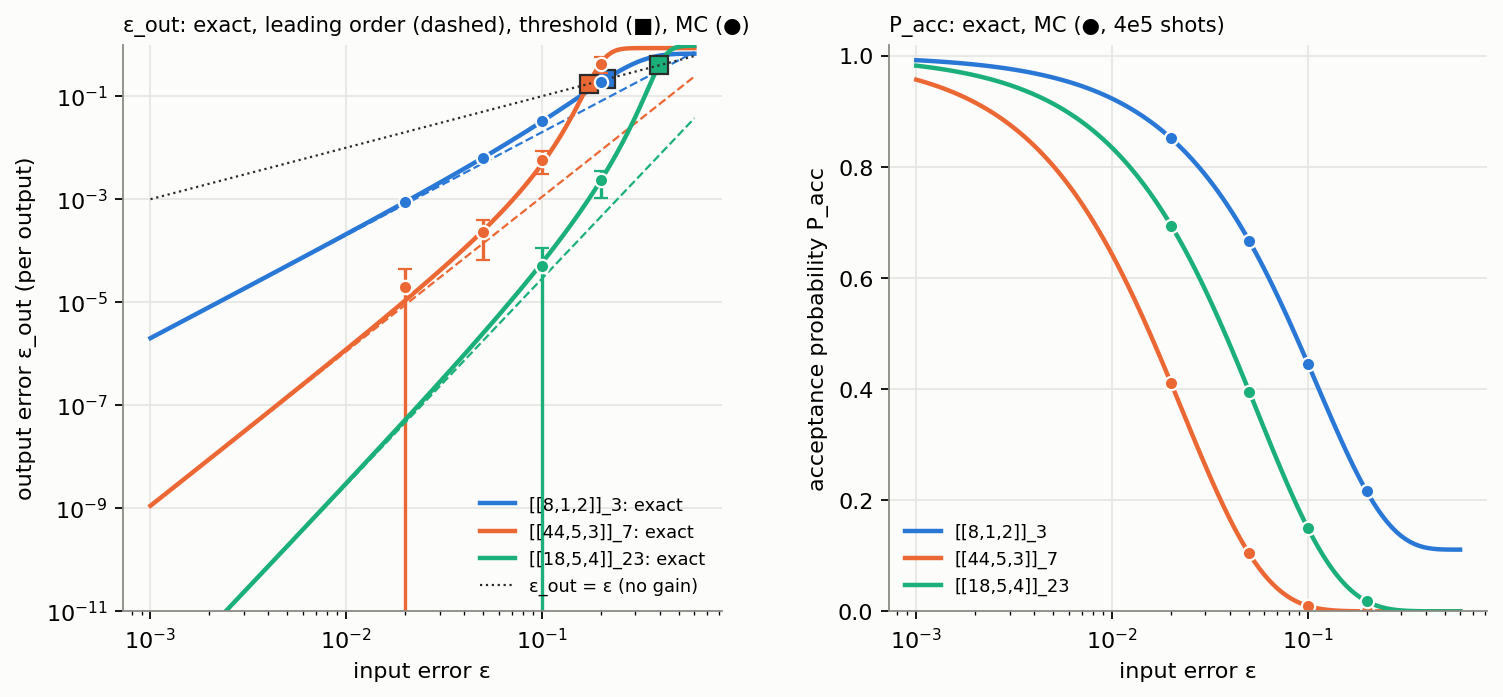
\includegraphics[width=\textwidth]{fig_curves.png}
\caption{Left: per-output error against input error for the three codes. Solid:
exact engine. Dashed: leading order $c\,\eps^d$. Square: threshold
$\eps_{\mathrm{out}}=\eps$. Dots with error bars: \code{mc\_distill.simulate} with
$4\times10^{5}$ shots at $\eps\in\{0.2,0.1,0.05,0.02\}$. Right: acceptance
probability, same conventions. Your first deliverable is this figure with your own
dots on it.}
\label{fig:curves}
\end{figure}

\begin{figure}[t]
\centering
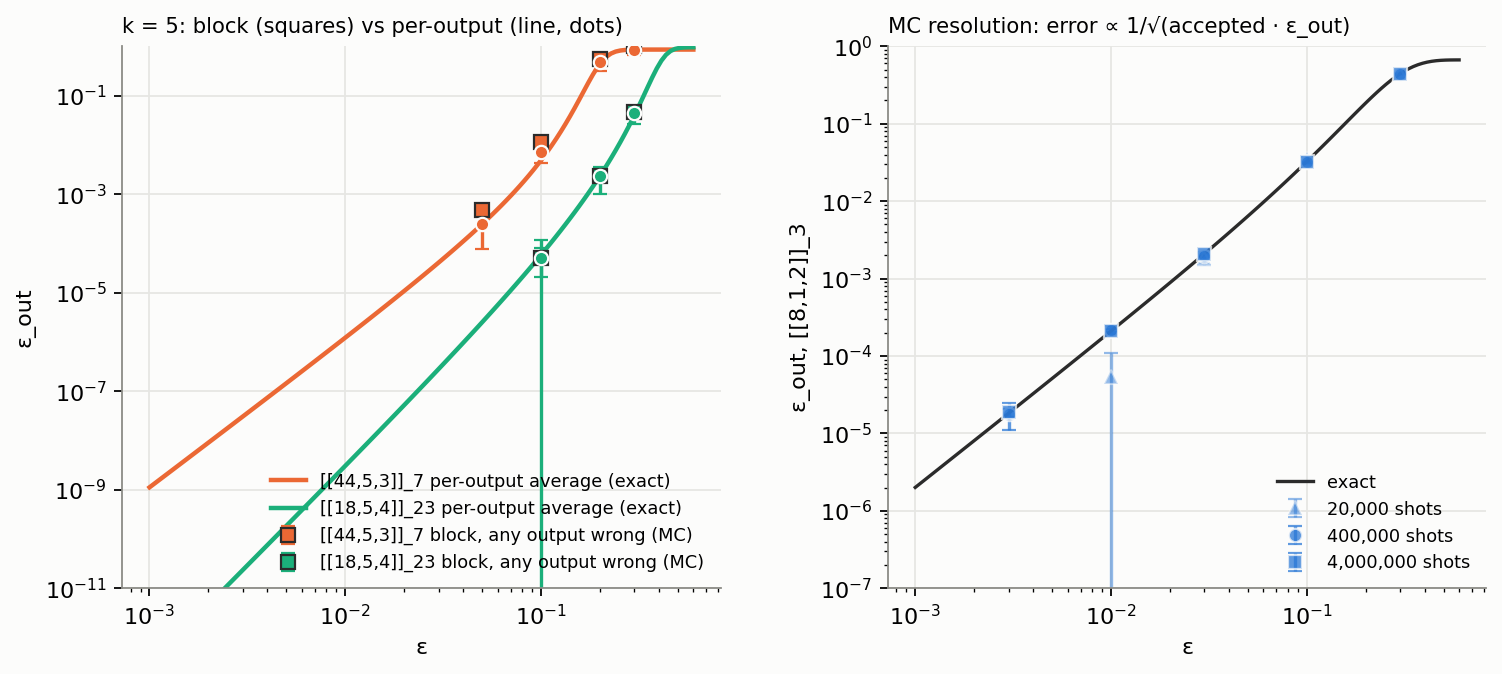
\includegraphics[width=\textwidth]{fig_block_and_shots.png}
\caption{Left: for the two $k=5$ codes, the block error (squares, Monte Carlo) sits
above the per-output average (line exact, dots Monte Carlo) and the ratio grows
toward $k=5$ as $\eps$ falls. Right: the sampler's resolution for $[[8,1,2]]_3$ at
$2\times10^{4}$, $4\times10^{5}$ and $4\times10^{6}$ shots; the error bar scales as
$1/\sqrt{(\text{accepted shots})\cdot\eps_{\mathrm{out}}}$, so each decade of
$\eps_{\mathrm{out}}$ costs a decade of shots.}
\label{fig:shots}
\end{figure}

How to read Figure~\ref{fig:curves}. On a log--log plot a power law $c\,\eps^{d}$
is a straight line of slope $d$; the dashed lines are those, and the solid exact
curves peel away from them upward as $\eps$ grows, because higher-order terms
($\eps^{d+1}$, $\eps^{d+2}$, \dots) stop being negligible. The dotted diagonal is
$\eps_{\mathrm{out}}=\eps$; a code only helps where its curve is below the diagonal,
and the square marks where it crosses. The Monte Carlo dots sit on the exact curve
where they have small error bars and become useless (huge bars, or missing
entirely) once $\eps_{\mathrm{out}}$ drops below roughly one over the number of
accepted shots.

\section{Inside \code{qmsd/mc\_distill.py}}
\label{sec:code}

The whole sampler is one function. Read it next to Section~\ref{sec:model}; every
line implements one sentence there.

\begin{lstlisting}
def simulate(G0, H1, p, eps, shots, seed=0, batch=200_000) -> dict:
    G0 = np.asarray(G0, dtype=np.int64) % p          # stabiliser rows, shape (dim A, n)
    H1 = np.asarray(H1, dtype=np.int64) % p          # logical rows,    shape (k, n)
    k, n = H1.shape
    rng = np.random.default_rng(seed)
    acc = hits = blk = 0
    done = 0
    while done < shots:
        b = min(batch, shots - done)
        # (1) the noise: each coordinate is nonzero w.p. eps, value uniform on 1..p-1
        j = np.where(rng.random((b, n)) < eps, rng.integers(1, p, size=(b, n)), 0)
        # (2) acceptance: every syndrome G0 j (mod p) must vanish
        ok = ~np.any((j @ G0.T) % p, axis=1)
        # (3) failure: for accepted shots, which outputs see the error?
        logical = ((j[ok] @ H1.T) % p) != 0           # shape (accepted, k), boolean
        acc += int(ok.sum())
        hits += int(logical.sum())                    # total wrong outputs
        blk += int(logical.any(axis=1).sum())         # shots with any wrong output
        done += b
    def frac(x, m):                                   # binomial estimate with 1-sigma error
        f = x / m if m else float("nan")
        return f, math.sqrt(f * (1 - f) / m) if m else float("nan")
    pa, pa_err = frac(acc, shots)                     # P_acc
    eb, eb_err = frac(blk, acc)                       # block error, conditioned on acceptance
    ea = hits / (k * acc) if acc else float("nan")    # per-output average
    ea_err = math.sqrt(max(ea * (1 - ea), 0.0) / acc) * math.sqrt(k) if acc else float("nan")
    return {...}
\end{lstlisting}

\paragraph{Line by line.}
\begin{itemize}[nosep]
\item \textbf{(1) Sampling the noise.} \code{rng.random((b, n)) < eps} is a boolean
  matrix of which qudits are hit; \code{rng.integers(1, p, ...)} draws the nonzero
  $Z$ power uniformly; \code{np.where} combines them. Each row of \code{j} is one
  error vector, i.e.\ one \emph{shot}.
\item \textbf{(2) Acceptance is a matrix product.} \code{j @ G0.T} computes every
  syndrome of every shot at once; \code{\% p} reduces mod $p$; \code{np.any(..., axis=1)}
  asks whether any syndrome is nonzero. There is no quantum state anywhere. That is
  what makes the channel-level model exact and fast, and it is exactly what
  \code{sdim} will put back.
\item \textbf{(3) Failure is a second matrix product.} Only accepted shots are kept
  (\code{j[ok]}); \code{logical[s, i]} is true if output $i$ of shot $s$ is wrong.
  \code{hits} counts wrong outputs (for the per-output average), \code{blk} counts
  shots with at least one (for the block error).
\item \textbf{Batching.} Shots are generated $2\times10^{5}$ at a time so memory stays
  at a few tens of MB however large \code{shots} is. \code{seed} makes a run
  reproducible; change it to get an independent sample.
\item \textbf{Error bars are binomial.} A count $x$ out of $m$ trials with true
  probability $f$ has standard deviation $\sqrt{f(1-f)/m}$. $P_{\mathrm{acc}}$ is a
  fraction of \code{shots}; the block error is a fraction of \emph{accepted} shots,
  which is why its bar is larger. The per-output average adds $k$ correlated
  indicators per shot, so its bar is bounded by $\sqrt{k}$ times the block-style
  estimate rather than computed exactly (Exercise~\ref{ex:errbar}).
\item \textbf{What is not modelled.} No gate noise, no measurement noise, no $X$
  errors (this code family does not post-select on them at all), no correlated
  noise, and no Clifford correction step. The sampler validates the engine's
  arithmetic under the engine's own assumptions; the circuit simulation tests the
  assumptions.
\end{itemize}

\begin{vocab}
\textbf{Monte Carlo}: estimating a probability by drawing random samples and
counting.
\textbf{Shot}: one random sample (here one error vector $j$ on $n$ qudits).
\textbf{Accepted shot}: a shot that passed post-selection; the conditional
probabilities are fractions of these, not of all shots.
\textbf{$1\sigma$ error bar}: one standard deviation of the estimator; a true value
should fall within $1\sigma$ about 68\% of the time, within $3\sigma$ 99.7\%.
\textbf{Importance sampling}: drawing from a distribution that over-represents the
rare events you care about and correcting each sample by a weight
(true probability divided by sampling probability), so the estimate is still
unbiased but far less noisy.
\end{vocab}

\section{Exercises}
\label{sec:ex}

Work in a scratch directory inside the repo, run everything with
\code{PYTHONPATH=.} from the repo root, and keep the memory cap
(\code{ulimit -v 4000000}) and single-thread BLAS (\code{OMP\_NUM\_THREADS=1}) on the
shared boxes. Write each result into a small JSON next to your script; the plots
come last. The exercises build on each other: 1--2 get you a working pipeline, 3--4
teach you what the numbers mean, 5--6 cover the two quantities the paper quotes, 7--9
improve the sampler, 10 applies it to your own codes.

\subsection*{Getting a point and a curve}

The first exercise is a smoke test: one code, one $\eps$, one number to compare. The
only ways to fail it are a wrong matrix (Appendix~\ref{app:matrices}), a wrong
convention for $\eps$, or a bug in your harness, so it is worth doing before anything
else.

\begin{exercise}{1: reproduce one point}
Build $[[8,1,2]]_3$ (Appendix~\ref{app:matrices}) and run
\code{simulate(G0, H1, 3, 0.05, shots=400\_000, seed=1)}.
\end{exercise}
\begin{checkbox}
$P_{\mathrm{acc}} = 0.6679$ and $\eps_{\mathrm{out}} = 6.40\times10^{-3}$. A run with
seed 1 gave $0.6671\pm0.0007$ and $6.33\times10^{-3}\pm1.5\times10^{-4}$. Anything
within about $3\sigma$ is a pass; a $5\sigma$ miss means a bug, not bad luck.
\end{checkbox}

A single point can agree by accident. A curve across two decades of $\eps$ and
three primes cannot, and it also shows you the shape of the problem: the steep
power-law region, the bend near threshold, and the point where sampling gives out.

\begin{exercise}{2: the whole curve}
Repeat for $\eps\in\{0.3,0.2,0.1,0.05,0.02,0.01\}$ and all three codes, and plot the
points over the exact curves (the exact curve is three lines of code,
Appendix~\ref{app:exact}). Use a log--log axis, one colour per code, error bars on
every point, and a legend.
\end{exercise}
\begin{checkbox}
Figure~\ref{fig:curves}. At $\eps = 0.02$ and $0.01$ the $[[18,5,4]]_{23}$ points will
be zero with a zero error bar: $4\times10^{5}$ shots cannot see $\eps_{\mathrm{out}}
\sim 10^{-8}$. That is correct behaviour, not a bug, and the next exercise
quantifies it.
\end{checkbox}

\subsection*{What the numbers mean}

The statistical error of a counting experiment is set by the number of events
counted, not by the number of trials. If $N_{\mathrm{acc}}$ shots are accepted and a
fraction $\eps_{\mathrm{out}}$ of them fail, you count about
$N_{\mathrm{acc}}\,\eps_{\mathrm{out}}$ failures, and the relative error of that
count is $1/\sqrt{N_{\mathrm{acc}}\,\eps_{\mathrm{out}}}$. Every decade you want to
push $\eps_{\mathrm{out}}$ down costs a decade of shots. This single fact decides
when simulation is the right tool and when the exact engine is.

\begin{exercise}{3: resolution and cost}
Show empirically that the relative error of $\eps_{\mathrm{out}}$ scales as
$1/\sqrt{N_{\mathrm{acc}}\,\eps_{\mathrm{out}}}$ by running $[[8,1,2]]_3$ at
$\eps=0.03$ with $2\times10^{4}$, $2\times10^{5}$, $2\times10^{6}$ shots. Then
estimate how many shots a 10\% measurement of $[[18,5,4]]_{23}$ at $\eps=0.01$ would
need.
\end{exercise}
\begin{checkbox}
Right panel of Figure~\ref{fig:shots}. For the estimate: $P_{\mathrm{acc}}=0.83$ and
$\eps_{\mathrm{out}}=3.1\times10^{-9}$, so 10\% needs about 100 failures, i.e.\
$3\times10^{10}$ accepted and $4\times10^{10}$ shots. At $\sim10^{6}$ shots per second
that is half a day for one point. This is why the engine exists, and why
Exercise~\ref{ex:is} matters.
\end{checkbox}

The distance is usually computed algebraically (our MITM kernels find the lightest
undetected error). It can also be \emph{measured}: on a log--log plot the
small-$\eps$ slope of $\eps_{\mathrm{out}}$ is $d$. Doing this once makes the
abstract definition concrete, and the discrepancy you will see at larger $\eps$ is
the higher-order terms the leading-order formula drops.

\begin{exercise}{4: distance and leading coefficient from data}
From your points at $\eps\in\{0.1,0.05,0.02\}$ fit $\log\eps_{\mathrm{out}}$ against
$\log\eps$ for $[[44,5,3]]_7$ (a straight line, weighted by the error bars). The slope
is the distance, the intercept the coefficient.
\end{exercise}
\begin{checkbox}
Slope $\approx 3$ (exactly $d=3$ only as $\eps\to0$; between 0.1 and 0.02 you should
see 2.8 to 3.0), coefficient $\approx 1.1$. The exact values are $d=3$,
$c_\eps = 1.111 = L_3/6^3$ with $L_3 = 240$ weight-3 accepted logical errors per
output.
\end{checkbox}

\subsection*{The two numbers the paper quotes}

Papers report a code's threshold and its block error. The threshold answers ``how
good must the raw magic states be for this code to help at all?''; it is a fixed
point of the map $\eps\mapsto\eps_{\mathrm{out}}(\eps)$. Near the fixed point
$\eps_{\mathrm{out}}-\eps$ is small and changes sign, so a sampler needs enough
shots to resolve the sign, which is harder than it sounds.

\begin{exercise}{5: threshold by bisection}
Find $\eps^{*}$ for $[[8,1,2]]_3$ as the root of $\eps_{\mathrm{out}}(\eps)-\eps$,
using the sampler at $10^{5}$ shots per evaluation. Think about why bisection needs
the sign of the difference and how many shots that requires near the root.
\end{exercise}
\begin{checkbox}
$\eps^{*}=0.2110$ (engine). The paper arXiv:2610.08012 Table~2 prints 0.211. Expect
$\pm0.003$ from the sampler.
\end{checkbox}

For $k>1$ the block error over-counts what a recursion pays for, by up to a factor
$k$. The sampler gives both notions from the same shots, so the ratio comes for free
and its $\eps$-dependence is a direct view of how many outputs a typical undetected
error touches.

\begin{exercise}{6: block against per-output}
For $[[44,5,3]]_7$ at $\eps\in\{0.3,0.1,0.05\}$ compute the ratio
$\eps_{\mathrm{out}}^{\mathrm{blk}}/\eps_{\mathrm{out}}^{\mathrm{avg}}$ from the
sampler's two estimates. Explain the trend.
\end{exercise}
\begin{checkbox}
Left panel of Figure~\ref{fig:shots}: the ratio is about 1.3 at $\eps=0.3$ and about
2.1 at $\eps=0.05$, heading to $k=5$. At high $\eps$ the accepted errors are heavy and
hit several outputs at once; at low $\eps$ a weight-3 error hits one output.
\end{checkbox}

\subsection*{Improving the sampler}

Now modify the code. Keep the original function untouched (the test suite uses it)
and work on a copy. The first improvement is honest statistics for the per-output
estimate: the shipped bar is a bound because the $k$ indicators of one shot are
correlated (an error that corrupts output 1 is more likely than average to corrupt
output 2 as well), and the clean way to handle correlated indicators is to treat
the per-shot count as the random variable.

\begin{exercise}{7: better error bars}\label{ex:errbar}
Modify a copy of \code{simulate} to accumulate, per accepted shot, the number of
wrong outputs $w\in\{0,\dots,k\}$ (its sum and its sum of squares), and compute the
variance of $w/k$ directly. Compare the new bar with the old one at $\eps=0.05$ for
$[[44,5,3]]_7$.
\end{exercise}
\begin{checkbox}
The new bar must be smaller than or equal to the old one and never below the
block-style bar divided by $\sqrt{k}$. Report both.
\end{checkbox}

The engine and the sampler meet in the weight distribution: the engine computes
exactly how many undetected errors there are of each weight, the sampler sees them
at the rate the noise produces them. Comparing the two bin by bin is the most
detailed check possible, and it is also how you would notice a subtle bug (a wrong
coset, a missed stabiliser) that the totals could hide.

\begin{exercise}{8: the weight histogram and MacWilliams}
Modify a copy of \code{simulate} to histogram the Hamming weight of every
\emph{accepted} $j$ and of every accepted $j$ that fails output 1. Compare the
low-weight bins, divided by the number of shots, against the engine's exact counts:
the number of accepted errors of weight $w$ is $B_w$ and the probability of one of
them is $(\eps/(p-1))^{w}(1-\eps)^{n-w}$.
\end{exercise}
\begin{checkbox}
For $[[8,1,2]]_3$: $L_2 = c_\eps (p-1)^d = 2\cdot 4 = 8$ weight-2 accepted logical
errors. Your weight-2 failing-bin frequency at $\eps=0.05$ must be
$8\,(0.025)^{2}(0.95)^{6} \approx 3.7\times10^{-3}$ of all shots, within error.
\end{checkbox}

Exercise~3 showed that direct sampling cannot reach small $\eps$: almost every shot
is error-free or lightly hit and accepted harmlessly, and the rare weight-$d$
failures never appear. Importance sampling fixes this by choosing the error weight
yourself. If you draw weight $w$ with probability $q_w$ and then a uniformly random
pattern of that weight, the true probability of that shot is $\binom{n}{w}
(\eps/(p-1))^{w}(1-\eps)^{n-w}$ divided by the number of patterns, and the shot gets
weight (true probability)/(sampling probability). Averages of weighted shots are
unbiased for any $q_w$ that gives nonzero probability to every relevant weight, and
putting most of $q_w$ on $w\in\{d,\dots,d+2\}$ is where the failures live.

\begin{exercise}{9: importance sampling}\label{ex:is}
Write a sampler that draws the error \emph{weight} $w$ from a distribution of your
choice, then a uniformly random pattern of that weight (positions and nonzero
values), and reweights each shot by the true probability $\binom{n}{w}(\eps/(p-1))^{w}
(1-\eps)^{n-w}$ divided by your proposal. Use it to measure $[[18,5,4]]_{23}$ at
$\eps=0.01$ and $0.001$. Report the effective sample size as well as the estimate.
\end{exercise}
\begin{checkbox}
$3.06\times10^{-9}$ at $\eps=0.01$. At $\eps=0.001$ compute the exact value yourself
with Appendix~\ref{app:exact}; it is close to $c_\eps\,\eps^{4} = 2.9\times10^{-13}$.
With $10^{6}$ reweighted shots concentrated on $w\in\{4,5,6\}$ you should get both to
a few percent.
\end{checkbox}

\subsection*{Your own codes}

Everything so far used codes whose exact curve is known. Your own catalog entries
are bigger. The engine can probably still enumerate $[[215,28,4]]_3$ ($3^{\dim A}$
with $\dim A$ in the twenties is borderline) but almost certainly not
$[[689,40,5]]_3$. For those the sampler is not a check on the engine; it \emph{is} the
performance number, and the only cross-check is the leading-order coefficient from
the $A_d$ count the search already recorded.

\begin{exercise}{10: your own codes}
Run Exercise~2 on your $[[215,28,4]]_3$ and $[[689,40,5]]_3$ entries. The exact engine
may refuse the larger one (too many words to enumerate; it says so). Then the
sampler is the only curve we have, and your points become the reference.
\end{exercise}
\begin{checkbox}
Where the engine runs, agreement as before. Where it does not, check your points
against the leading order $A_d/(p-1)^d\cdot\eps^{d}$ from the catalog's $A_d$ at the
two smallest $\eps$ you can resolve, and say in your write-up which regime you are in.
\end{checkbox}

\section{Toward the circuit simulation}
\label{sec:sdim}

The channel model assumes that the only noise is an independent $Z$ error on each
input magic state, delivered before a perfect circuit. A real round also has noisy
Clifford gates in the encoder, noisy syndrome measurements, idle errors while
qudits wait, and $X$-type errors that this family does not post-select on. The
question for \code{sdim} is how much each of these shifts the curve, and in which
direction. Before writing any circuit, write down what you expect:

\begin{itemize}[nosep]
\item A gate error rate $p_g$ adds terms to $\eps_{\mathrm{out}}$ that are
  \emph{first order} in $p_g$ and independent of $d$: a single faulty gate late in the
  circuit can corrupt an output without any syndrome firing. On a log--log plot
  against $\eps$ the curve therefore flattens into a floor at small $\eps$, and the
  floor height is the number to report. Predict it from the gate count and $p_g$
  before you simulate it.
\item Measurement errors change $P_{\mathrm{acc}}$ more than $\eps_{\mathrm{out}}$:
  a wrong syndrome mostly rejects good rounds (lower yield) rather than accepting
  bad ones.
\item The channel-level curve is the $p_g\to0$ limit. Your first \code{sdim} run should
  reproduce Exercise~1 with all circuit noise switched off; if it does not, the
  circuit is wrong, not the engine.
\end{itemize}

Start with $[[8,1,2]]_3$ (8 qutrits, two stabilisers, one logical) and then
$[[18,5,4]]_{23}$ if \code{sdim} supports $p=23$; $[[44,5,3]]_7$ is the realistic
target. The encoding circuit comes from $G_0$ and $H_1$ by the standard
CSS-encoder construction; ask before building it so we agree on the gate set.

\begin{vocab}
\textbf{Stabiliser simulator} (\code{sdim}): simulates Clifford circuits with Pauli
noise efficiently by tracking stabilisers instead of amplitudes; exact for
everything in a distillation round except the magic states themselves, which enter
as inputs.
\textbf{Gate error rate} $p_g$: probability that a gate is followed by a random
Pauli on its qudits.
\textbf{Floor}: the $\eps$-independent part of the output error caused by circuit
noise.
\end{vocab}

\section{Deliverables and checklist}

\begin{enumerate}[nosep]
\item \code{runs/mc/<code>\_<eps>.json} per point (shots, seed, all four estimates and
  errors), produced by a script committed under \code{scratchpad/} or \code{docs/}.
\item Figure~\ref{fig:curves} redrawn with your points, at least four codes, the
  three above plus one of yours.
\item A half-page note: which points agree, the measured scaling of
  Exercise~3, the fitted $d$ and $c$ of Exercise~4, and the importance-sampling
  result of Exercise~9.
\item Open a pull request against \code{main} from your branch. Leave the
  \code{primepower\_msd/} directory untouched.
\end{enumerate}

\appendix

\section{Getting $G_0$ and $H_1$}\label{app:matrices}

For a catalog record:
\begin{lstlisting}
from qmsd.results import load_result_catalog
from qmsd.performance import record_matrices
wanted = "imported-p23-n18-k5-4cc848da1772"
rec = next(r for r in load_result_catalog() if r.artifact_id == wanted)
G0, H1 = record_matrices(rec)      # integer arrays mod p; shapes (dim A, n) and (k, n)
\end{lstlisting}
For the $k=1$ Reed--Muller code $[[8,1,2]]_3$ (puncture one column of RM$(1,2)$ over
$\F_3$; any column is equivalent):
\begin{lstlisting}
from qmsd.reedmuller import r_max, rm_generator
from qmsd.triorthogonal import build_triorthogonal_code
from qmsd.performance import canonical_logical_rows
p, m = 3, 2
r = r_max(m, p); G = rm_generator(r, m, p)
G0 = build_triorthogonal_code(p, m, r, [1], G=G)["G0"]
H1 = canonical_logical_rows(G, [0], p)
\end{lstlisting}

\section{The exact curve in three lines}\label{app:exact}

\begin{lstlisting}
from qmsd.performance import profile_exact, leading_order, threshold
prof = profile_exact(G0, H1, p, kinds=("avg",))  # p**dim(A) words
print(float(prof.p_accept(0.05)), float(prof.eps_out(0.05, "avg")))
lo = leading_order(prof, "avg"); th = threshold(prof, "avg")
print(lo.d, lo.c_eps, th.eps)
\end{lstlisting}
The block kind (\code{kinds=("avg","block")}) costs $p^{\dim A + k}$ words and is
refused above $5\times10^{7}$; for $k=5$ at $p=23$ that is already too many, which
is why the block error in Figure~\ref{fig:shots} comes from the sampler.

\section{Files}

\begin{itemize}[nosep]
\item \code{qmsd/mc\_distill.py} is the sampler and \code{qmsd/performance.py} the
  exact engine. The test suite compares them in \code{tests/test\_performance.py}
  (\code{test\_monte\_carlo\_agrees}).
\item \code{PERFORMANCE.md}: the engine's write-up and validation against
  arXiv:2610.08012 Table~2. \code{COVERAGE.md}: the per-prime table of codes.
\item \code{docs/aanha\_mc\_guide/make\_figures.py}: produced every figure and number in
  this document; run it to regenerate them.
\end{itemize}

\end{document}
